\chapter{研究内容}

\section{研究目标}

本课题针对MoE模型带来以上挑战,拟分析现有的MoE模型分布式训练系统存在的缺陷,并设计一套全新的MoE模型训练系统。

MoE模型在分布式训练中面临几个挑战。首先,MoE模型的稀疏激活特性与现有的静态并行策略不匹配,导致计算资源无法充分利用。其次,MoE模型引入了全局所有GPU之间同步的All-to-All通信,严重影响训练速度和效率。最后,由于Gating策略的动态变化,节点负载可能不均衡,导致训练时间延长和模型性能下降。因此,需要采用动态并行策略、优化通信开销和实现负载均衡,以克服这些挑战,提高MoE模型的训练效率和性能。

如图\ref{fig-overview}所示,我们提出了一种全新的MoE训练系统,通过在算法层面(gating policy)和系统层面(Expert placement scheduler)提出创新的训练解决方案,旨在克服MoE模型训练过程中的瓶颈,并更好地适应复杂而庞大的深度学习任务需求。
\begin{figure}[h!]
    \vskip 2ex
    \centering
    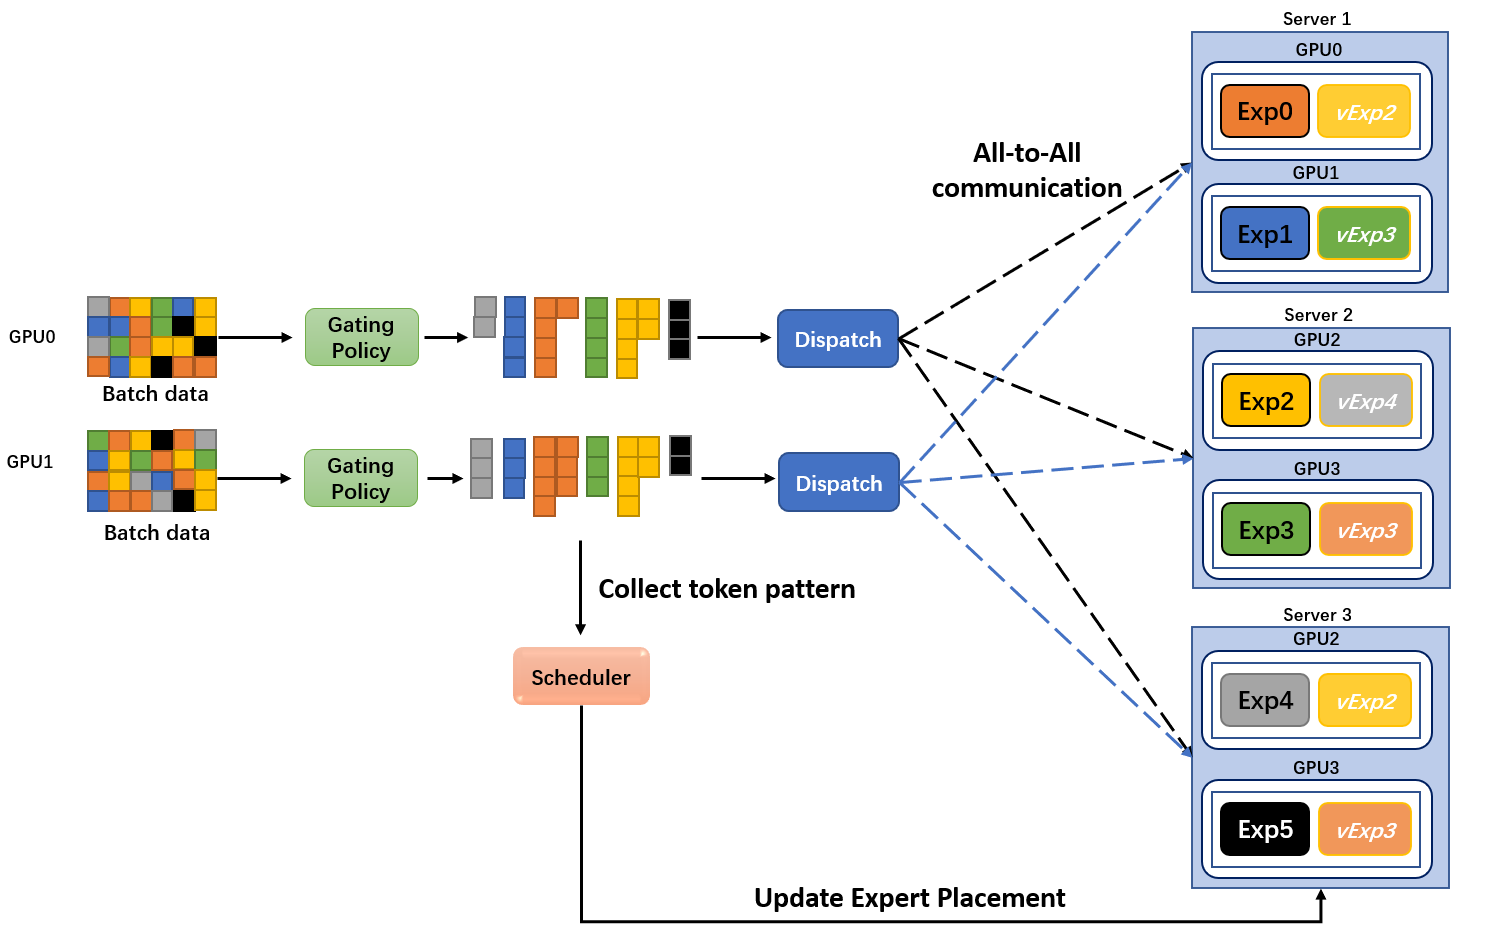
\includegraphics[width=0.99\linewidth]{figures/fig7.png}
    \caption{传统的Top1和Top2 Gating策略}
    \label{fig-overview}
    \end{figure}


我们的训练系统综合考虑了多个因素,包括任务特性、训练系统的拓扑结构、训练数据的分布以及每个专家的能力。通过算法与系统的协同设计,我们致力于实现能够动态优化专家的分布式并行策略,使每个专家都能够发挥最大潜力,并在整个系统中平衡负载和资源利用率。

在算法层面上,我们对MoE模型的数据分派关键部分,即gating策略,进行了改进。通过动态调整数据分派策略,我们实现了更快的收敛速度,并同时控制了全局通信开销。我们采用了All-to-All通信原语中的unequal模式,进一步减少由填充(padding)引起的额外数据发送量,从而降低全局通信的成本。

同时,在系统层面上,我们提出了一种基于网络拓扑的自动负载均衡策略。我们根据训练系统实际的网络拓扑结构,研究了不同拓扑结构下的数据传输和通信开销,并针对性地设计了一种优化策略。通过充分利用数据的局部性和专家之间的并行计算能力,我们能够减少通信开销,提高整体训练效率。
% 
我们的设计在offline的过程中,首先根据系统的网络拓扑结构,分析训练系统中任意两点进行通信操作的开销,并建立数学模型。
% 
在online过程中,我们设计了一种调度器(Expert placement scheduler),它能够收集并监测每一个MoE层中所有专家的任务负载。
% 
当检测到专家的负载发生一定变化时,调度器会根据当前负载情况和专家的放置情况,自动寻找最合适的专家并行放置策略,从而解决MoE模型在训练过程中由于负载动态变化而导致的训练效率低下的问题。
% 

这种全新的训练解决方案使得MoE模型能够更好地应对复杂和庞大的深度学习任务需求。通过优化算法和系统设计,我们能够充分发挥MoE模型的潜力,提高模型的准确性和泛化能力,为解决现实世界中的复杂问题提供有力工具。我们的研究对推动MoE技术的发展和应用具有重要意义,也对分布式训练系统的进一步发展起到推动作用。

\subsection{基于动态路由的数据分派策略}

\begin{figure}[h!]
\vskip 2ex
\centering
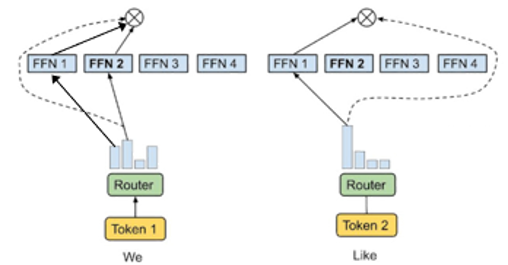
\includegraphics[width=0.5\linewidth]{figures/fig3.png}
\caption{传统的Top1和Top2 Gating策略}
\label{fig-top1_top2}
\end{figure}

如图\ref{fig-top1_top2}所示在传统的MoE模型中,采用固定的Top1和Top2 Gating策略,即将数据发送到分数最高(次高)的expert进行处理。
% 
然而,采用Top1 Gating时,由于只选择一个最高分数的expert,可能会错过其他有价值的信息,导致模型收敛速度较慢;
% 
而采用Top2 Gating时,虽然可以选择两个最高分数的expert,但每轮训练时间较长,因为需要进行两次All-to-All通信。
% 
因此我们能否将Top1和Top2 Gating策略结合起来,以一种动态的方式选择合适的数据分派策略,从而实现较快的收敛速度和较短的训练时间。
% 
一种简单的方法是,将每个数据按照Top1和Top2的分数进行排序,然后将它们分别分配给Top1和Top2的expert进行处理。
% 
这种方法可以利用Top1和Top2的优点,避免错过其他有价值的信息,同时减少通信开销,提高训练效率。

\subsection{基于网络拓扑的自动负载均衡策略}


\begin{figure}[t!]
\vskip 2ex
    \begin{minipage}[h]{0.48\linewidth}
        \centering
        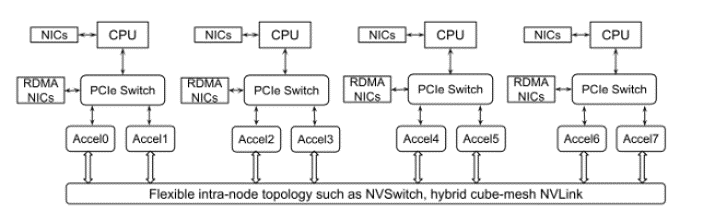
\includegraphics[width=1\linewidth]{figures/fig4.png}
        \caption{GPU集群内网络拓扑连接图}
        \label{fig-kek-tree}
    \end{minipage}
    %
    \begin{minipage}[h]{0.48\linewidth}
        \centering
        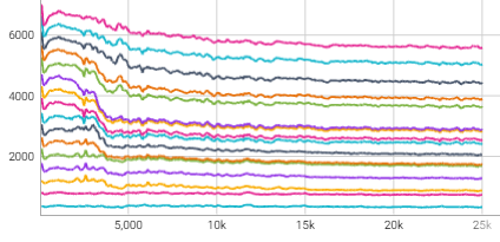
\includegraphics[width=0.8\linewidth]{figures/fig5.png}
        \caption{8层128专家的Transformer-XL\ucite{dai2019transformer}的MoE模型,第1层16个专家负载变化情况}
        \label{fig-transformer-xl}        
    \end{minipage}
\end{figure}

虽然基于 MoE 的算法开辟了一个巨大扩展模型参数量机会,但它也对训练系统带来了新的挑战,而这些挑战在之前的密集型DNN训练算法和系统中从未见过。根本原因是动态专家选择和灵活的 MoE 结构。具体来说,每个 MoE 层由一定数量的并行专家组成,这些专家分布在加速器(本工作中的 GPU)上,其中每个 GPU 根据智能门函数将每个输入数据分配给几个最适合的专家并取回相应的输出以将它们组合起来。这意味着每个专家的工作量基本上是不确定的,取决于输入数据和门函数。在图\ref{fig-transformer-xl}中,我们使用了一个8层的Transformer-xl MoE模型,分析了第1层16个专家负载变化情况。

我们发现,在MoE模型中,不同专家的负载在每次迭代中都会发生变化。
% 
这种现象是由于MoE的稀疏性动态数据分配所导致的,导致每个专家获取的数据不均匀,从而产生了负载不均衡的问题。
% 
这会导致一些节点或expert的负载过重,从而影响整个模型的训练速度和效果。因此,需要采取适当的负载均衡策略来缓解这个问题。
% 
此外在MoE模型中所有专家都需要从其他GPU上那里获得输入,这引入了GPU集群所有节点间额外的All-to-All通信,且All-to-All通信与后续计算是完全同步关系,并行较差。
% 
而GPU集群内部节点之间的网络带宽并不相同,节点通信效率存在差异。
% 
因而All-to-All通信也成为了大规模MoE训练中最耗时的操作之一。
% 
它通常实现为具有可变消息大小的同步 All-to-All 操作。考虑到动态特性的数据分派会导致计算和通信的严重不平衡,这样的方法会导致严重的开销。

因此,为了解决负载不均衡问题,需要采取一些适当的负载均衡策略,我们需要结合GPU集群内部节点之间的网络带宽不相同的情况,选择最佳的负载均衡策略,以提高整个模型的训练效率和性能。

% \medskip
\section{本章小结}

本章中,我们介绍了本项目对MoE模型的研究内容和研究目标。我们分析了MoE模型在分布式训练系统中的挑战,并介绍了设计的全新MoE模型训练系统。该系统在算法层面和系统层面提出了创新的训练解决方案,旨在克服MoE模型训练过程中的瓶颈,并更好地适应复杂而庞大的深度学习任务需求。

\endinput